\subsection{Quick Overview of Parallel Hardware}

\begin{frame}
\begin{block}{Three Basic Flavors of Hardware}
    
\includegraphics[width=0.95\textwidth]%
{../common/pics/hardware/ParallelHardware1.pdf}
\end{block}
\end{frame}

\begin{frame}
\begin{block}{Your Laptop or Desktop}
    
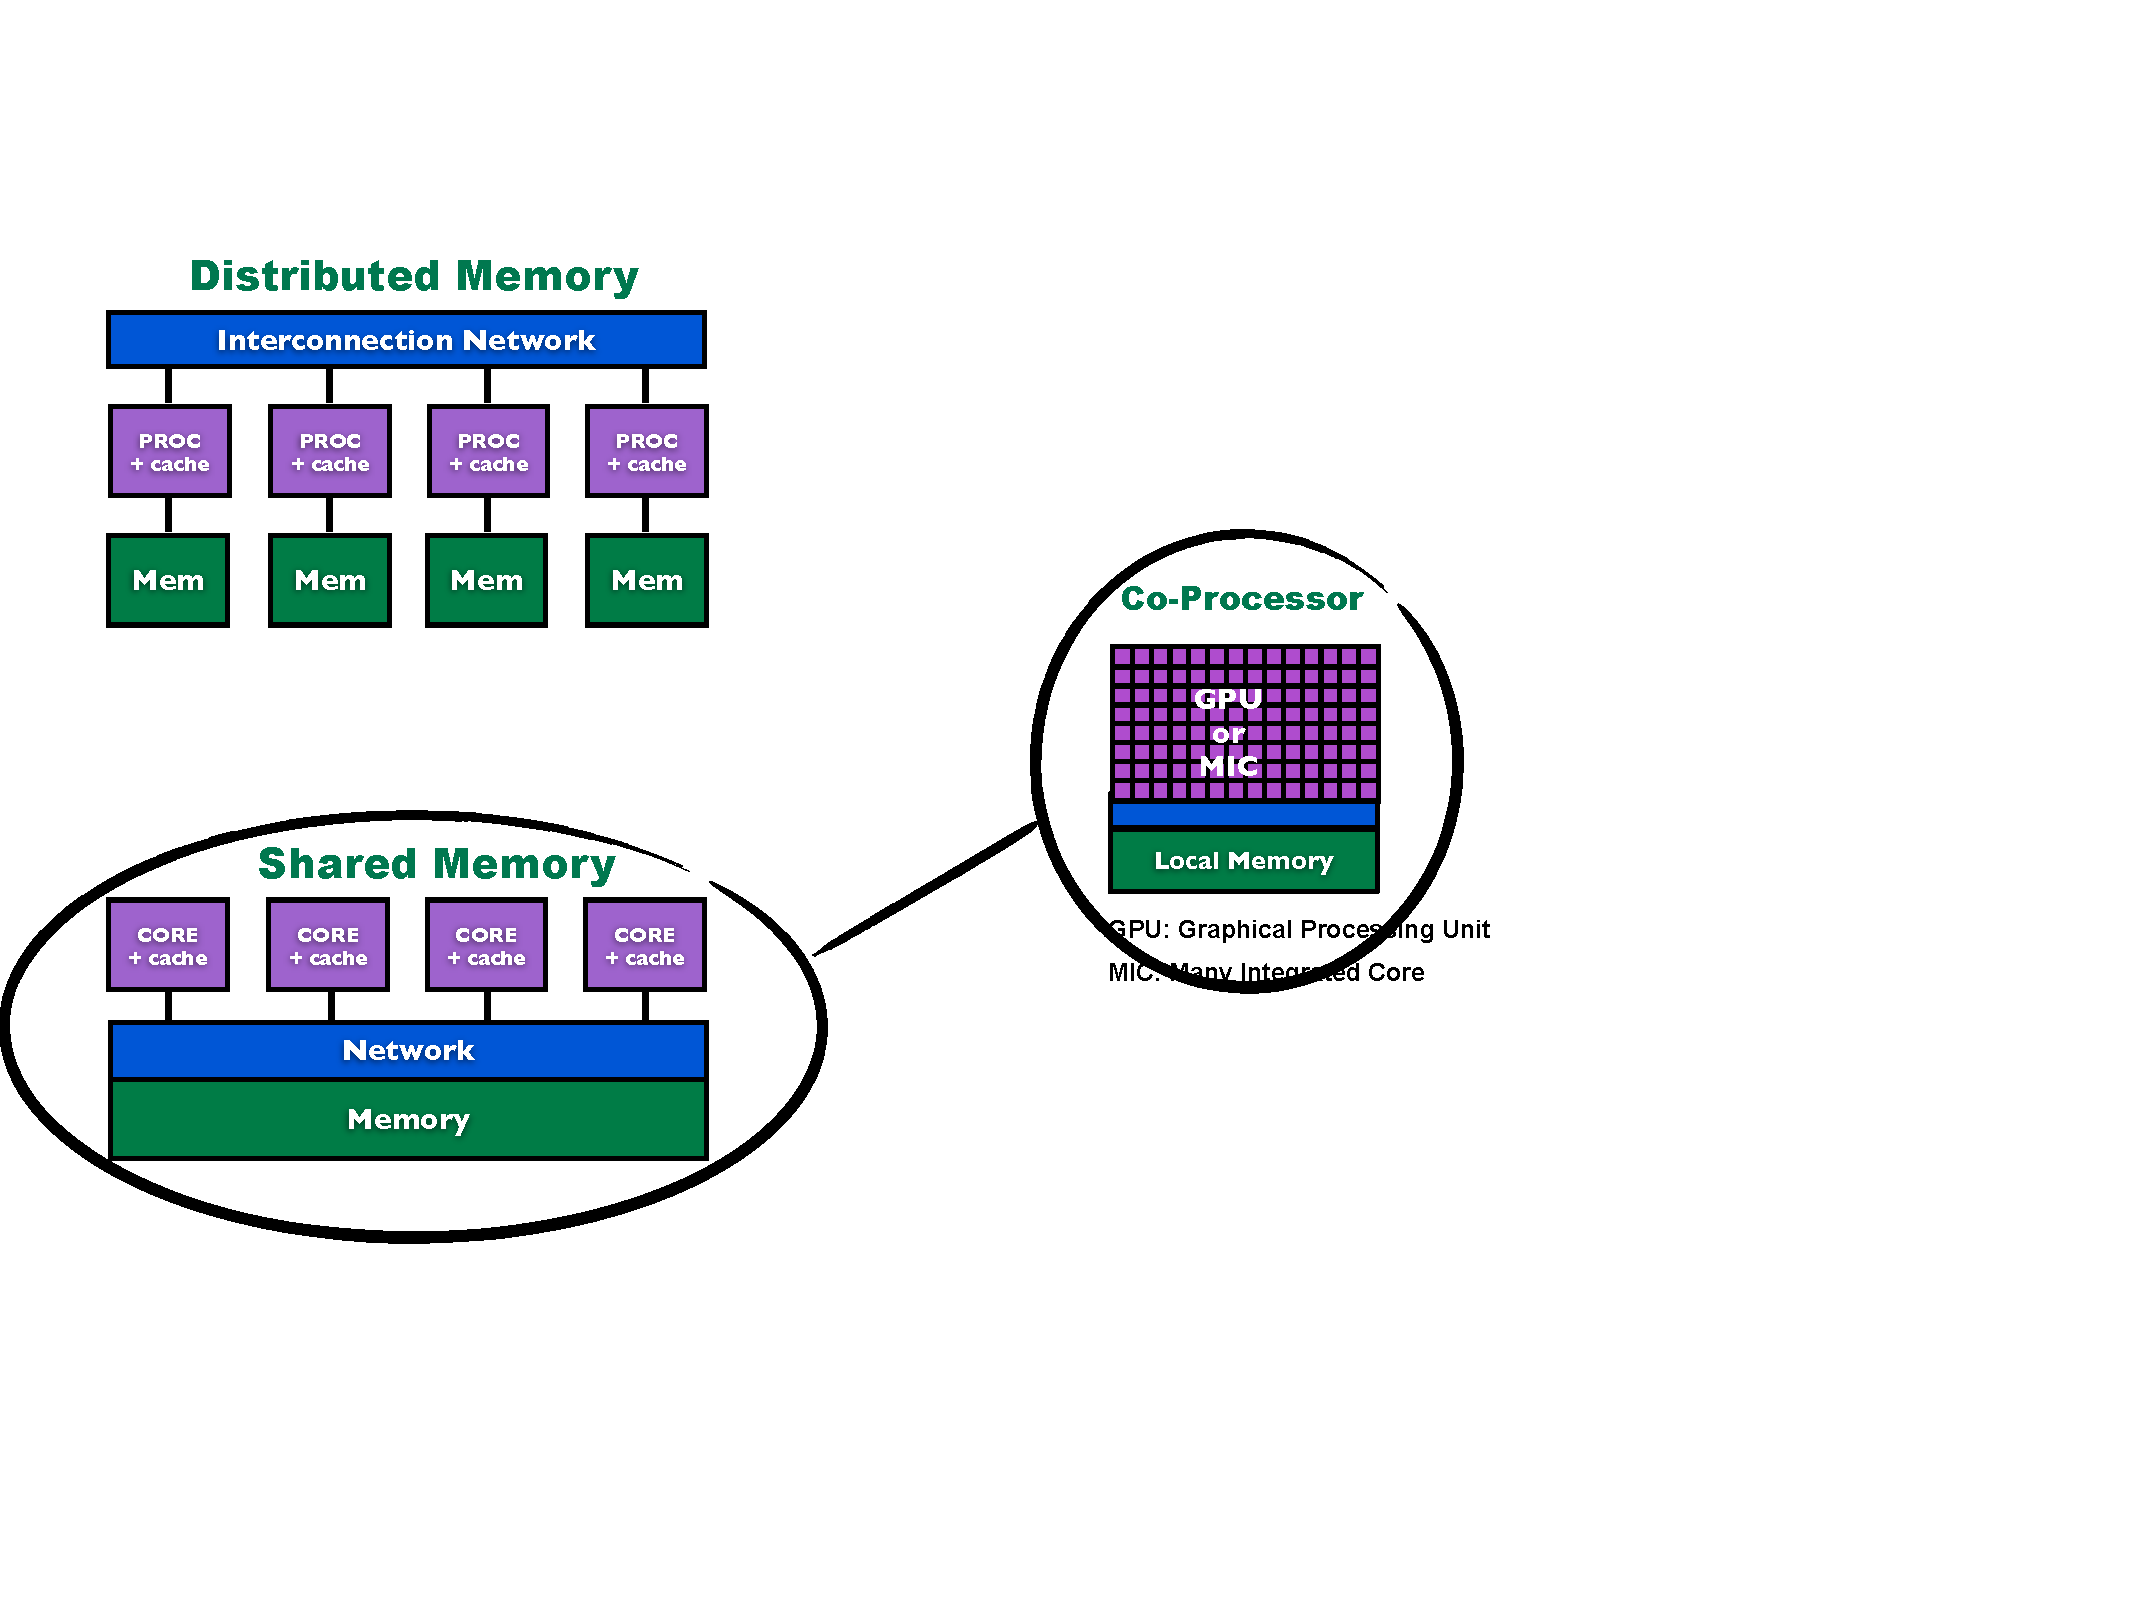
\includegraphics[width=0.95\textwidth]
{../common/pics/hardware/ParallelHardware2.pdf}
\end{block}
\end{frame}

\begin{frame}
\begin{block}{A Server or Cluster}
    
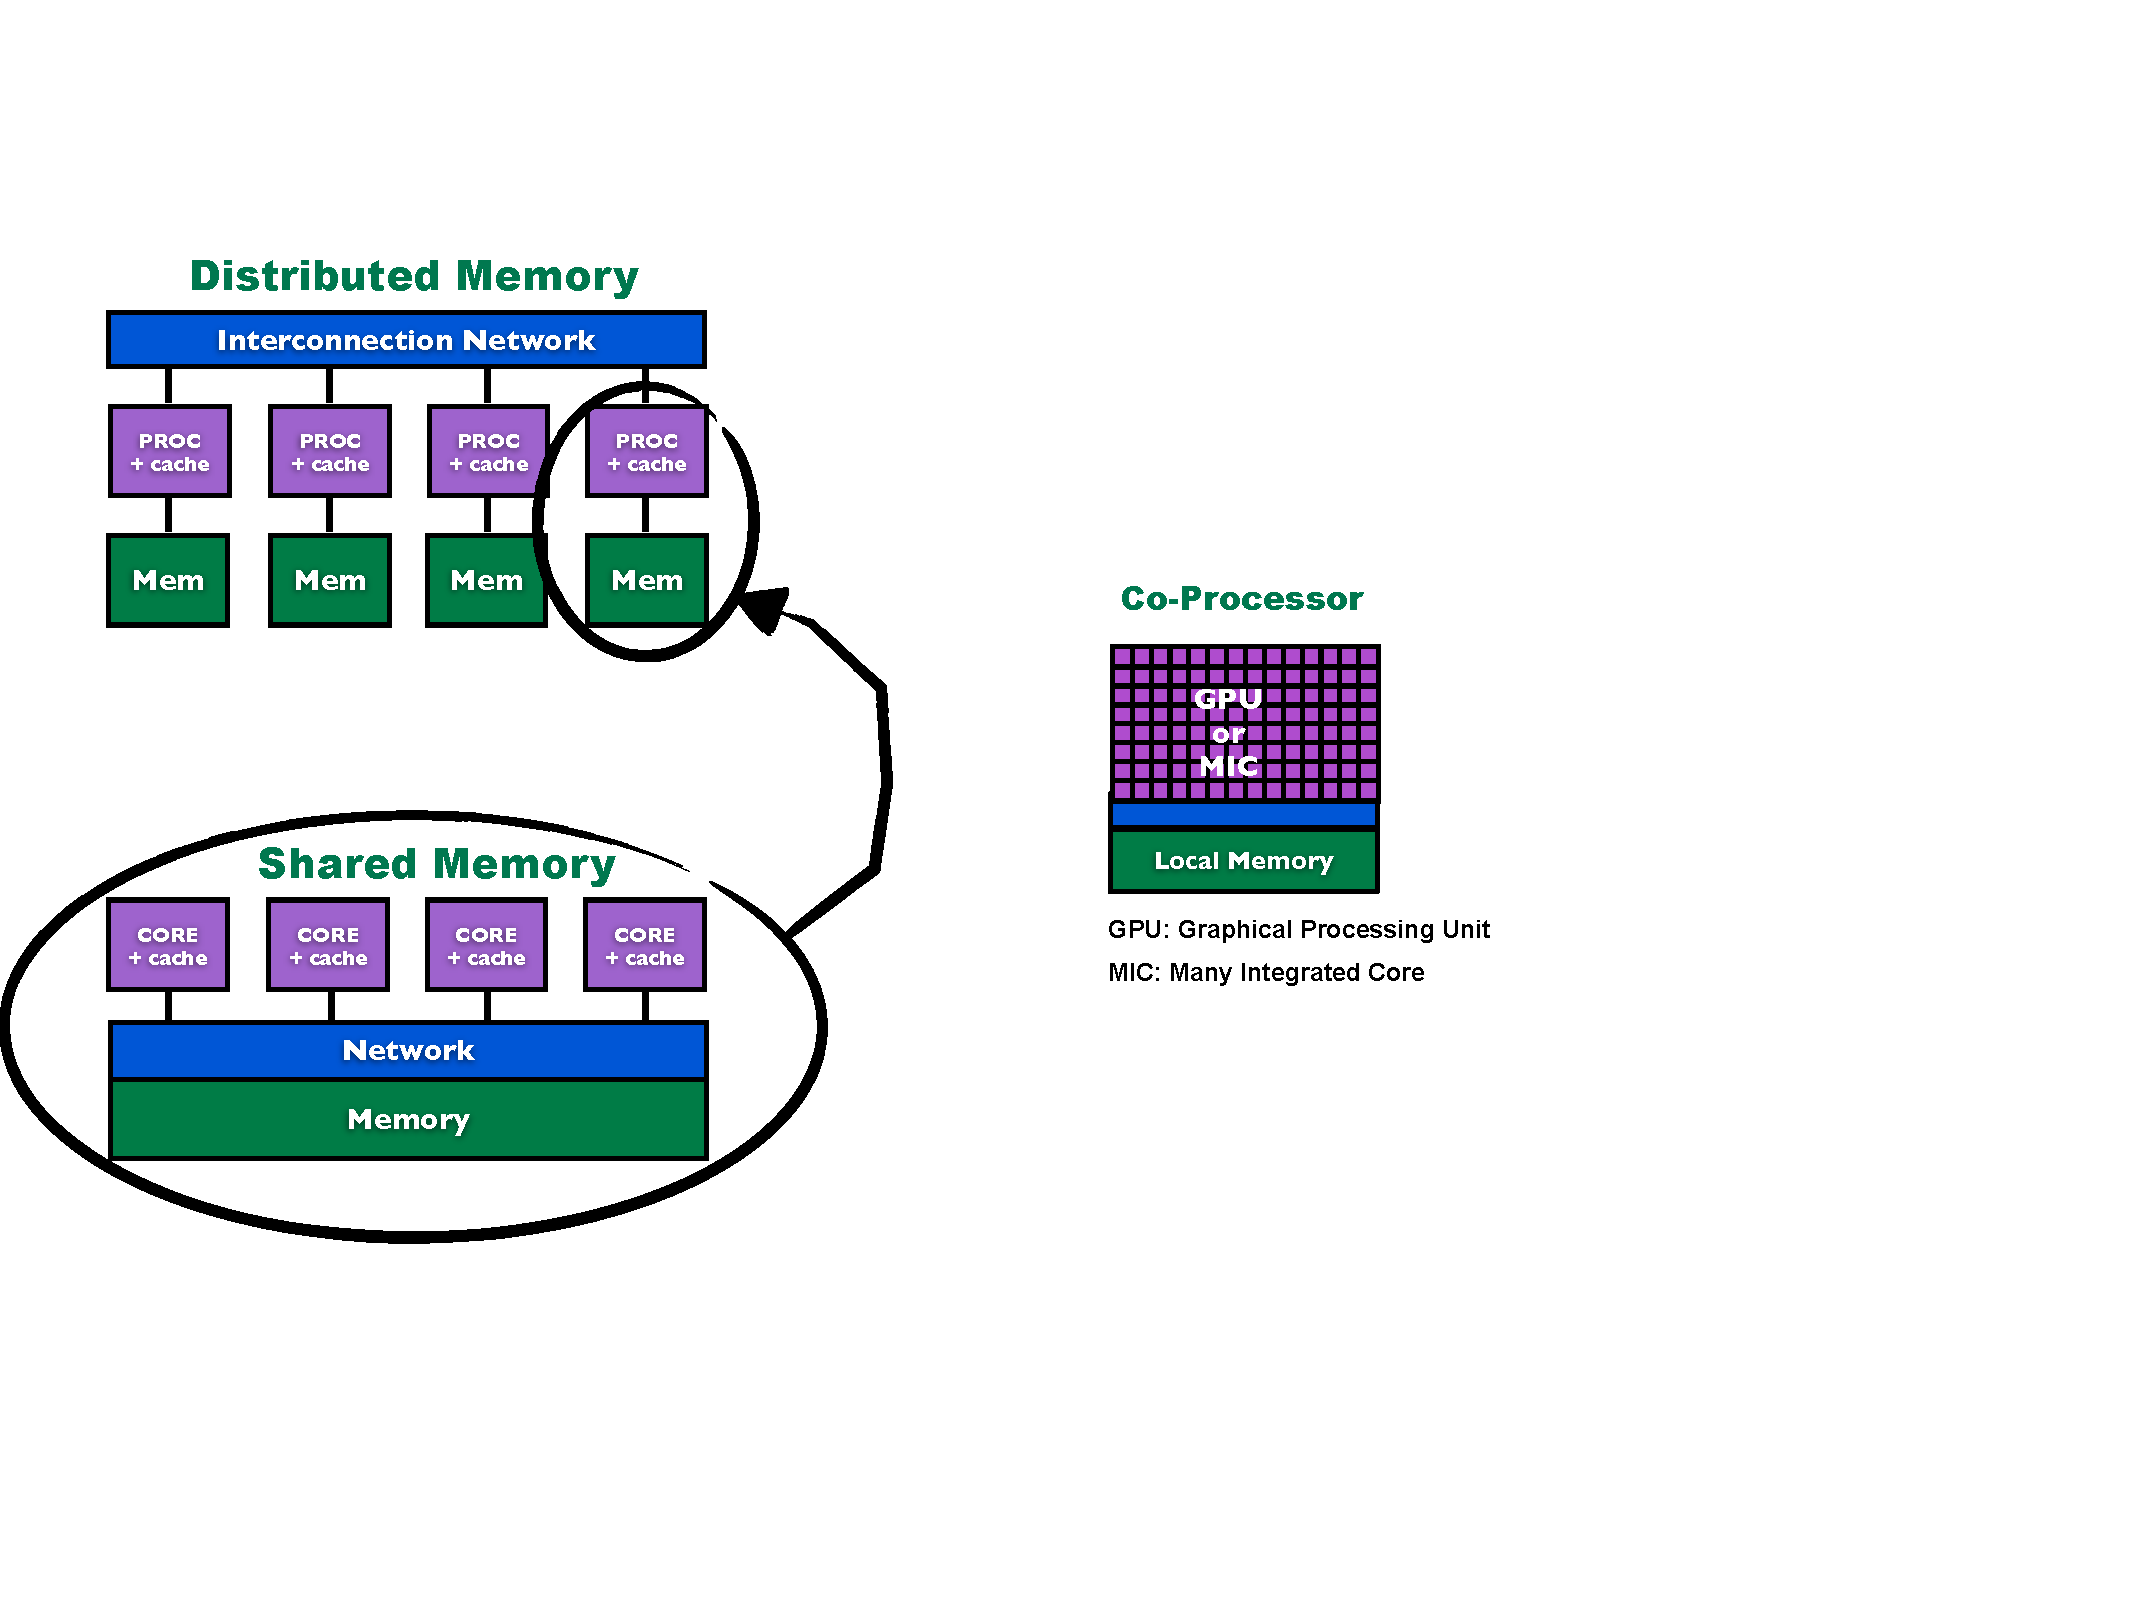
\includegraphics[width=0.95\textwidth]
{../common/pics/hardware/ParallelHardware3.pdf}
\end{block}
\end{frame}

\begin{frame}
\begin{block}{Server to Supercomputer}
    
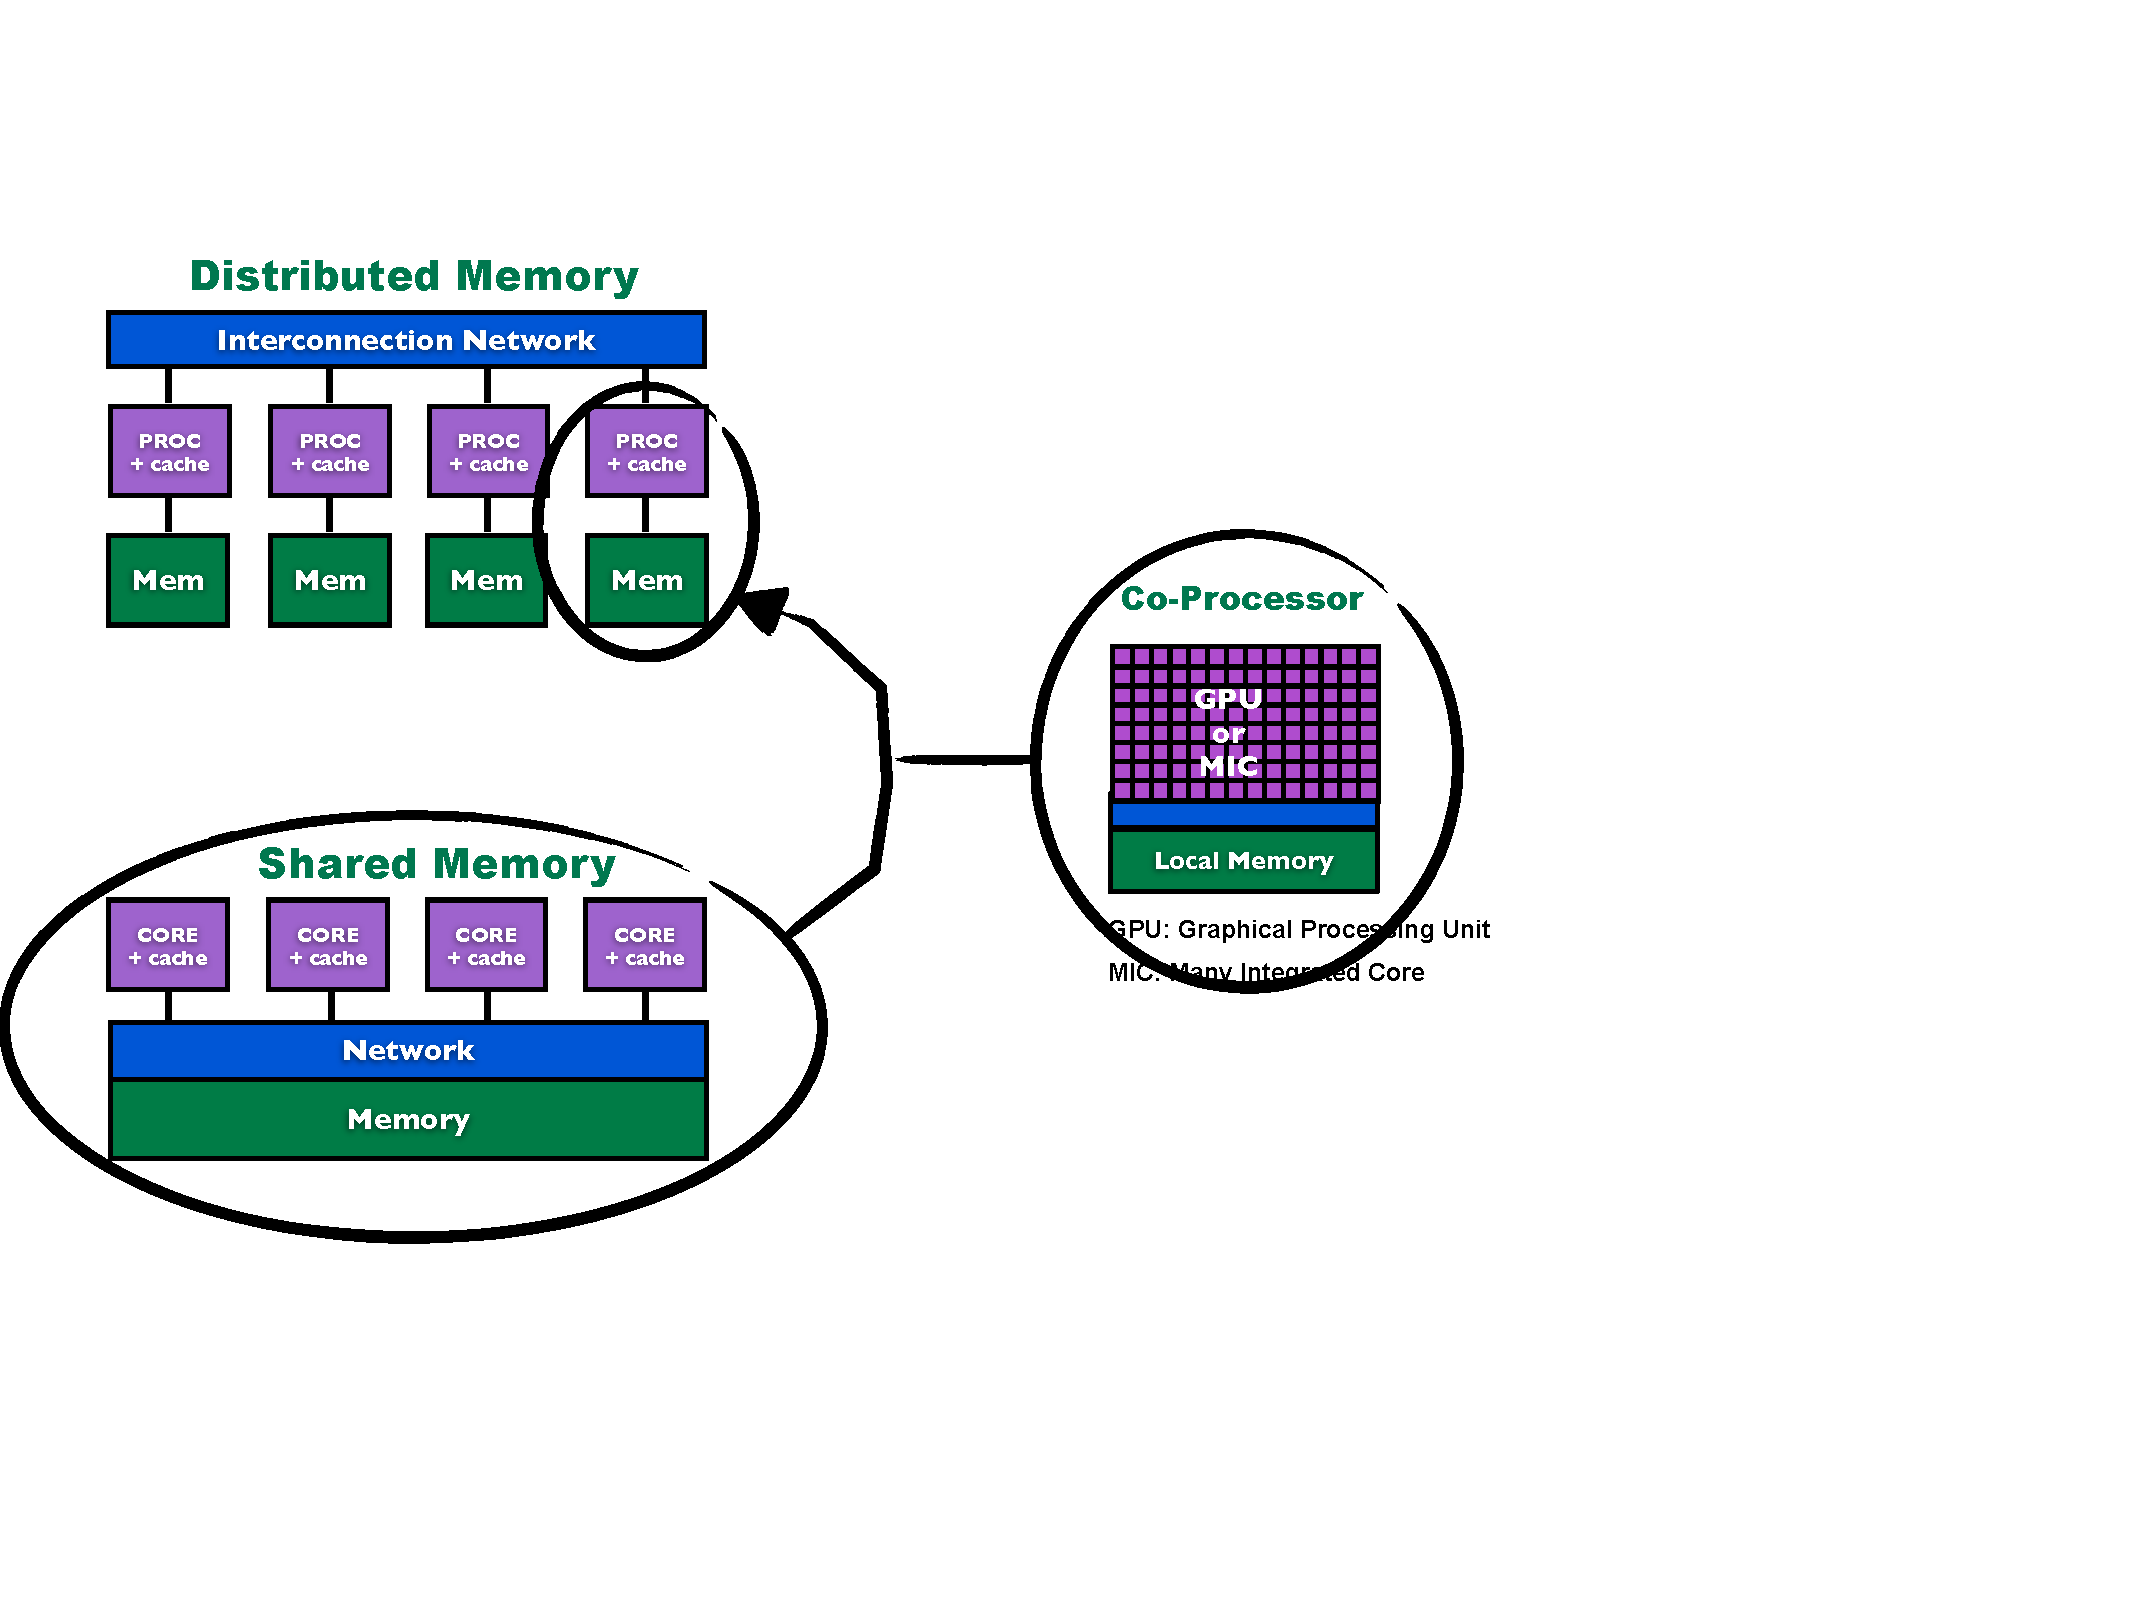
\includegraphics[width=0.95\textwidth]
{../common/pics/hardware/ParallelHardware4.pdf}
\end{block}
\end{frame}

\begin{frame}
\begin{block}{Knowing the Right Words}
    
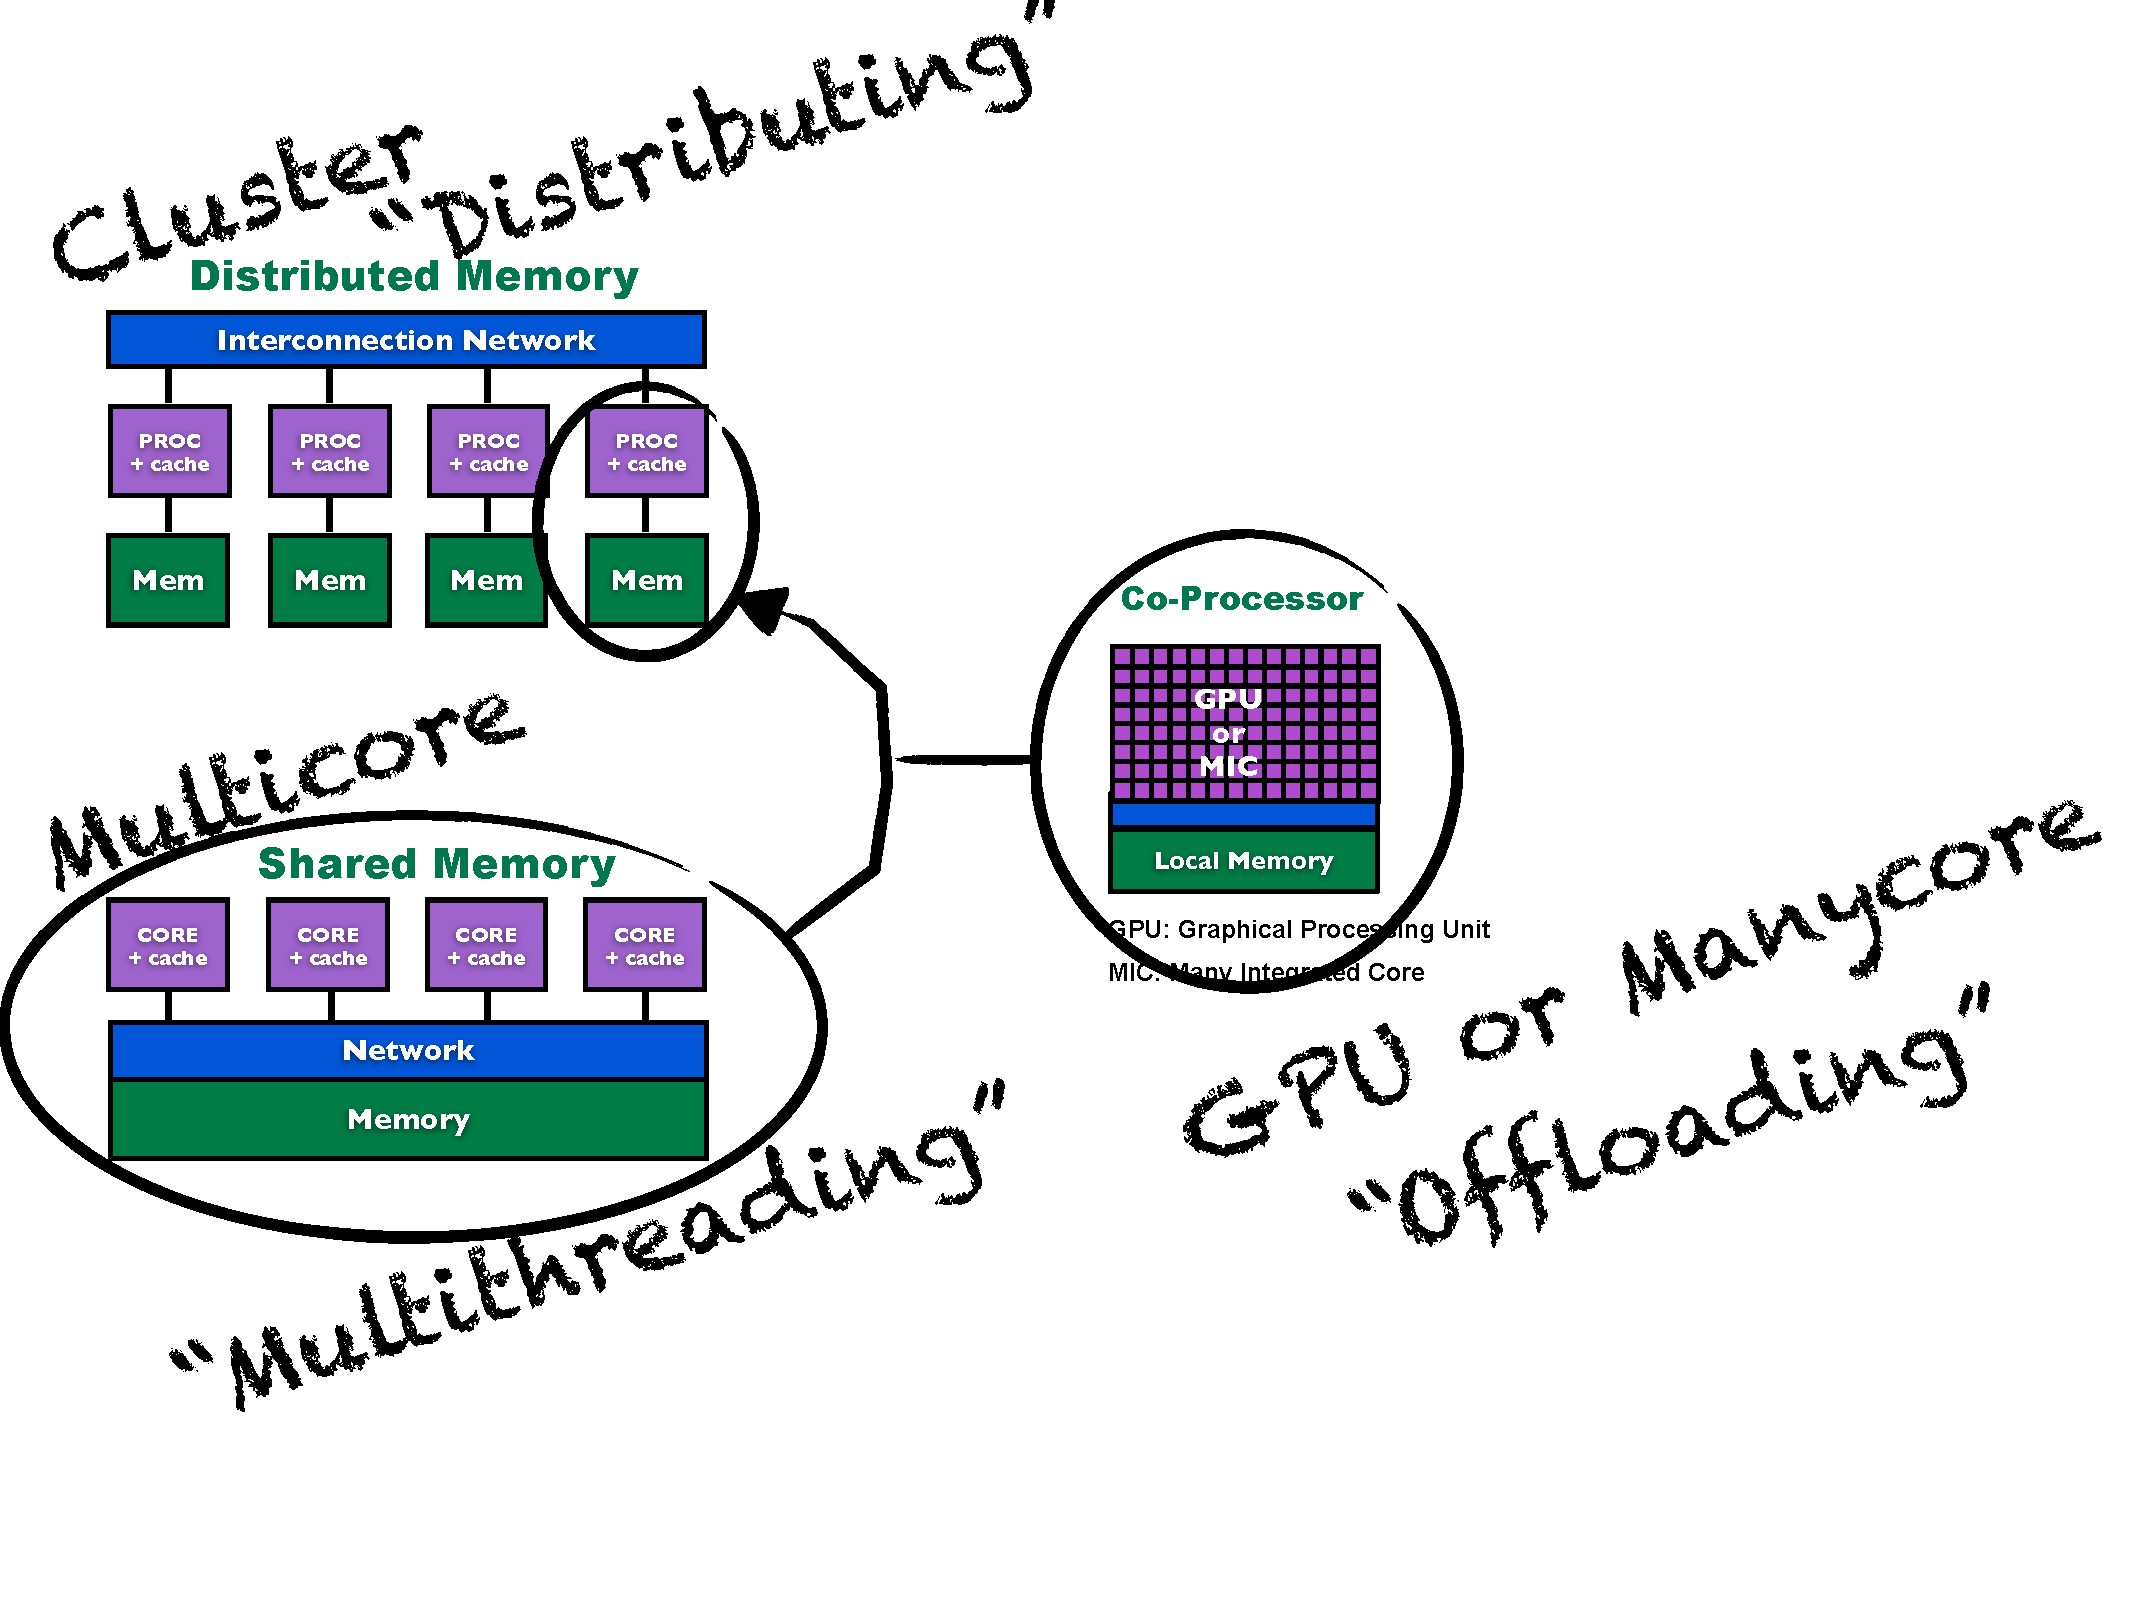
\includegraphics[width=0.95\textwidth]
{../common/pics/hardware/ParallelHardware5.pdf}
\end{block}
\end{frame}

\begin{frame}
\begin{block}{``Native'' Programming Models and Tools}
    
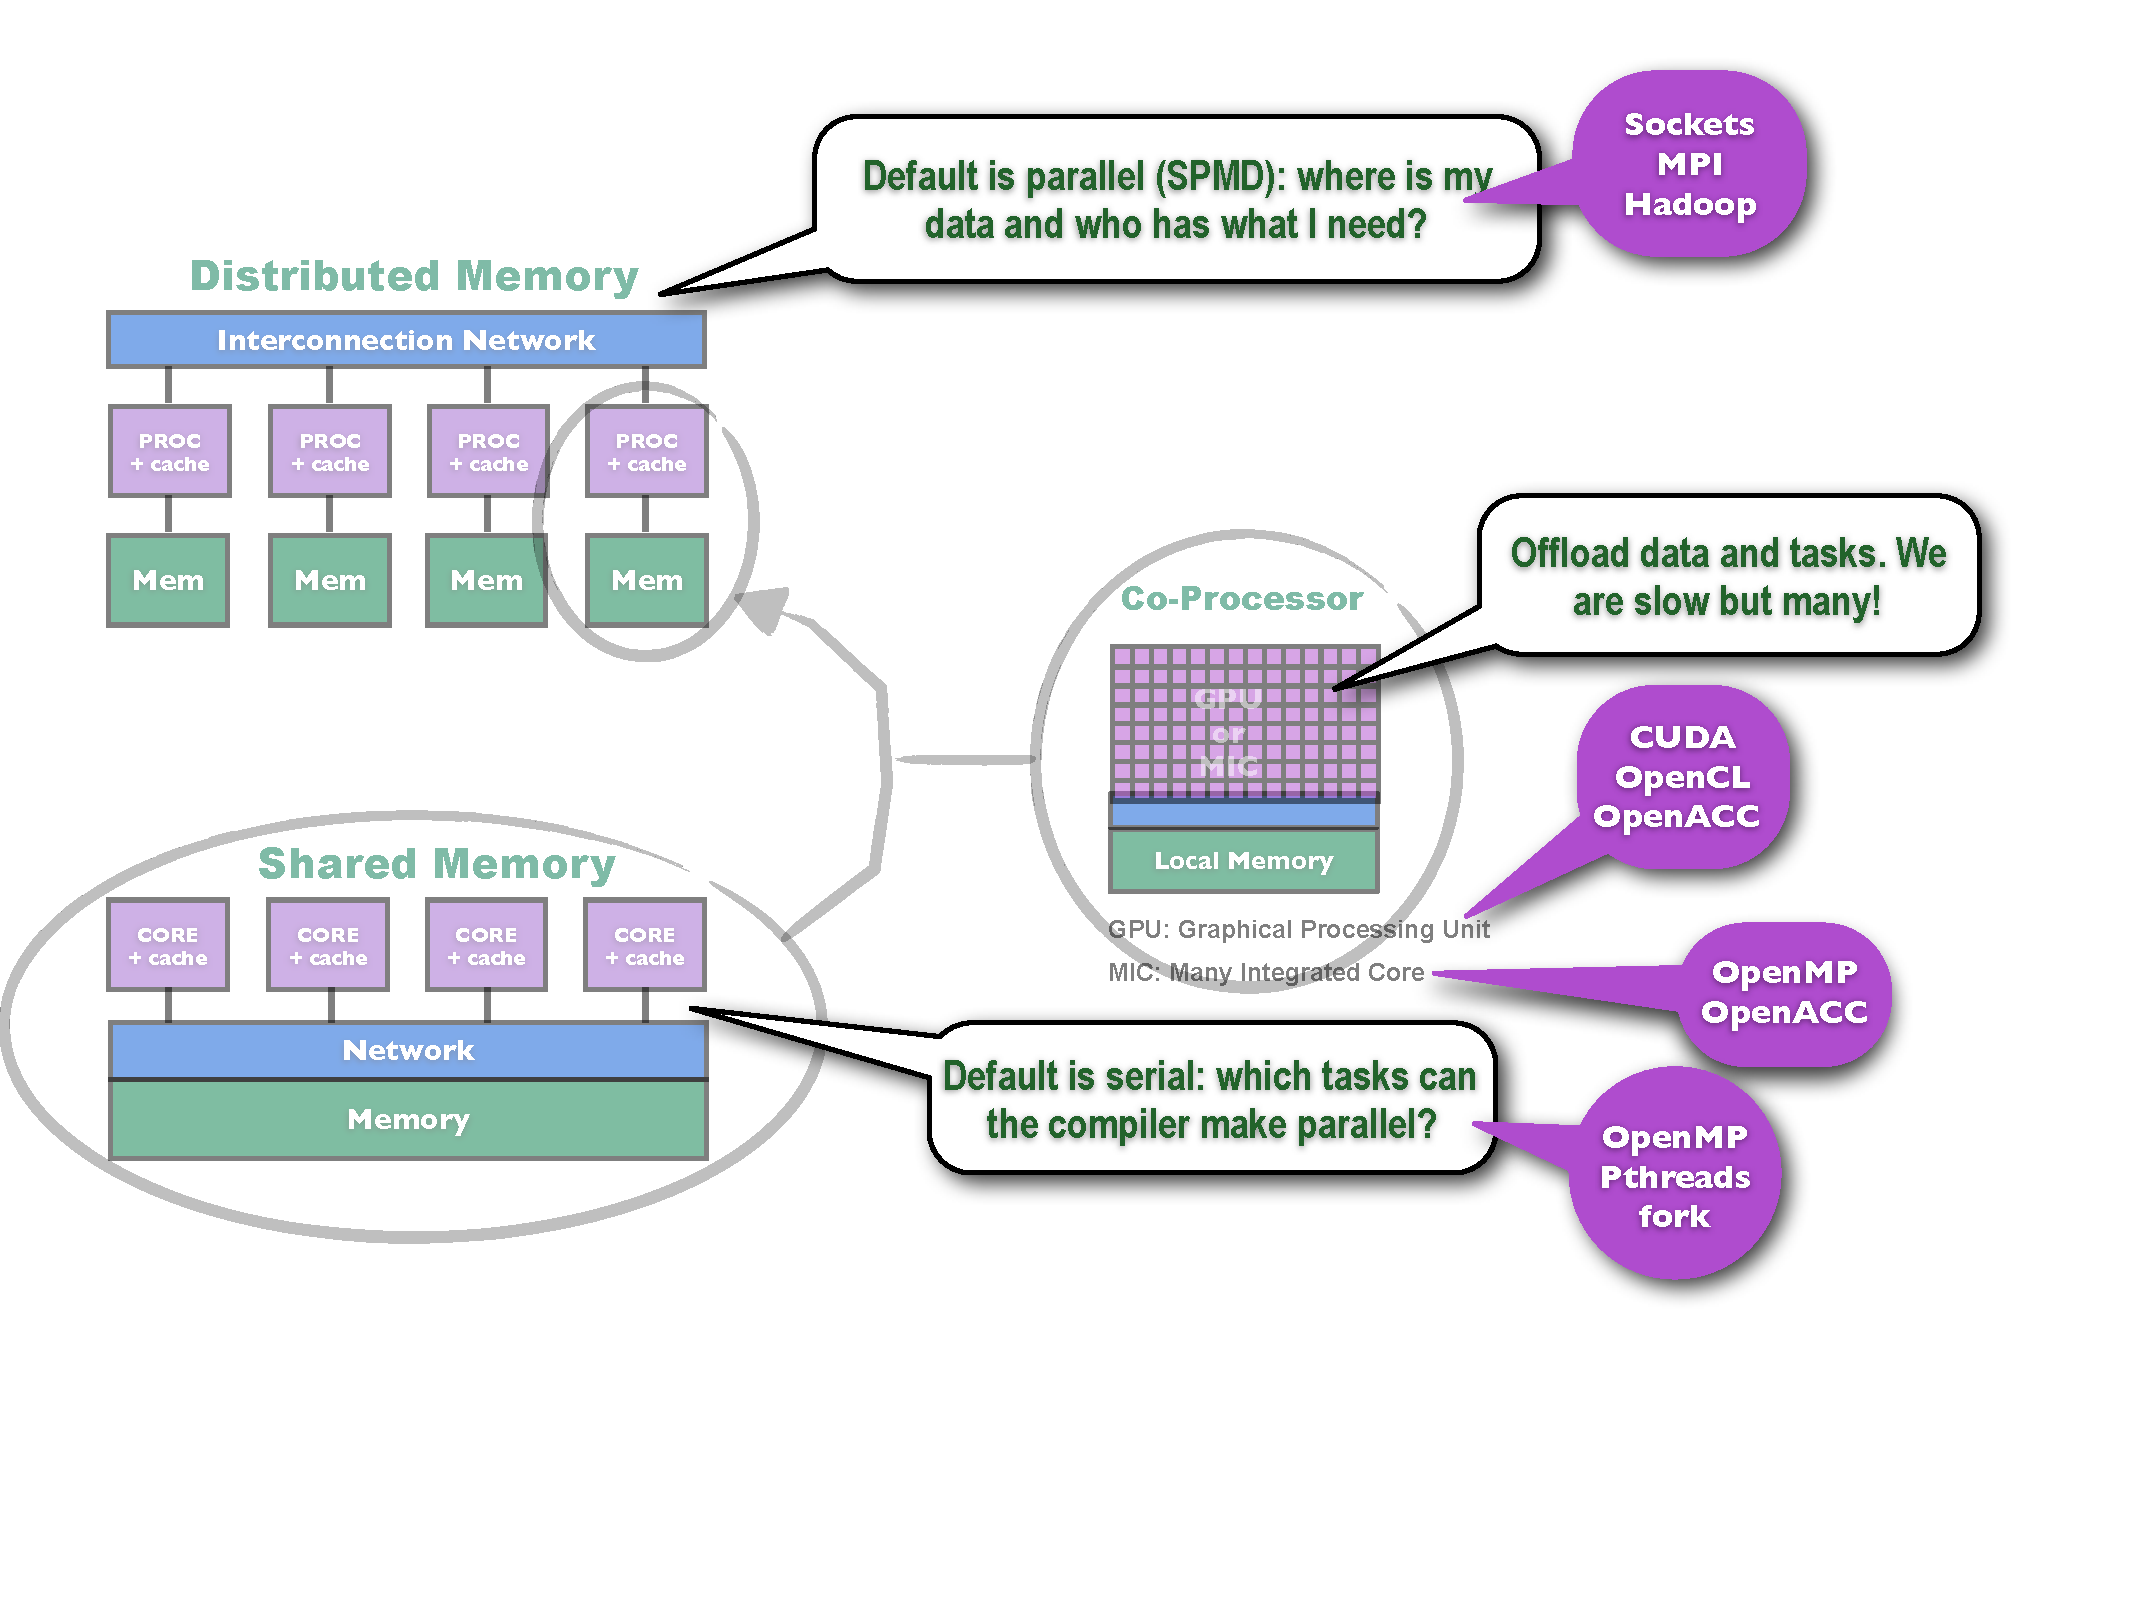
\includegraphics[width=0.95\textwidth]
{../common/pics/hardware/ParallelHardware6.pdf}
\end{block}
\end{frame}

\begin{frame}
\begin{block}{R Interfaces to Native Tools}
    
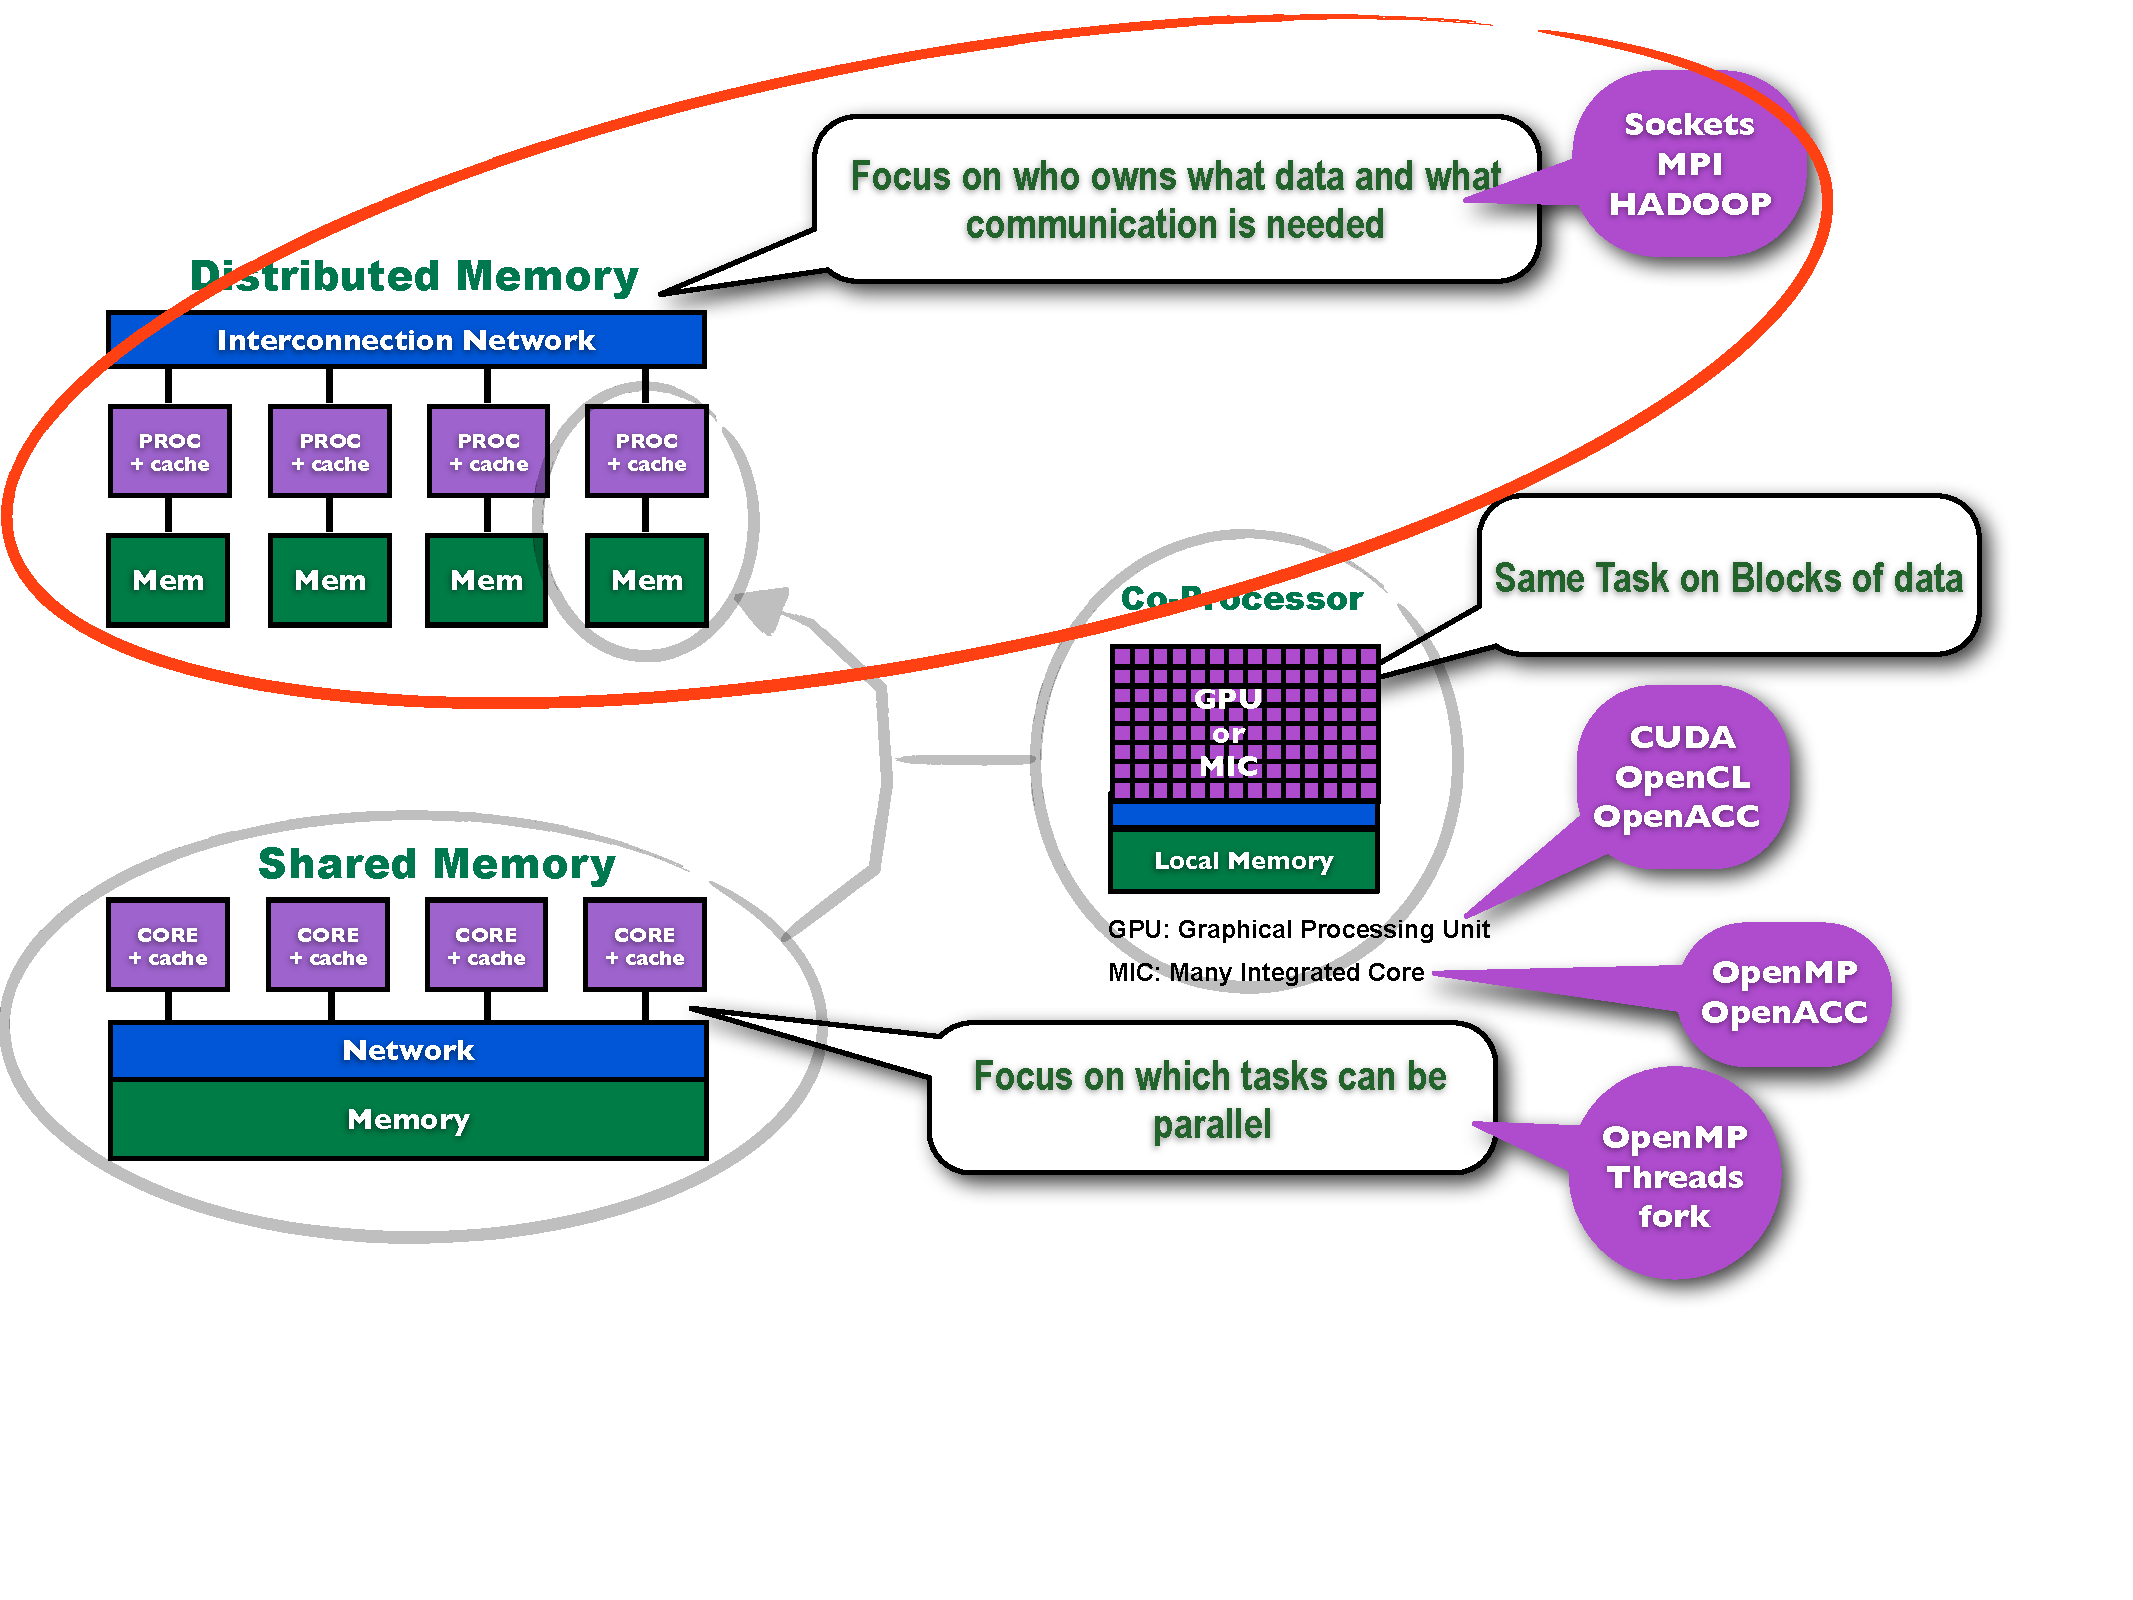
\includegraphics[width=0.95\textwidth]
{../common/pics/hardware/ParallelHardware7.pdf}
\end{block}
\end{frame}

\begin{frame}
\begin{block}{30+ Years of Parallel Computing Research}
    
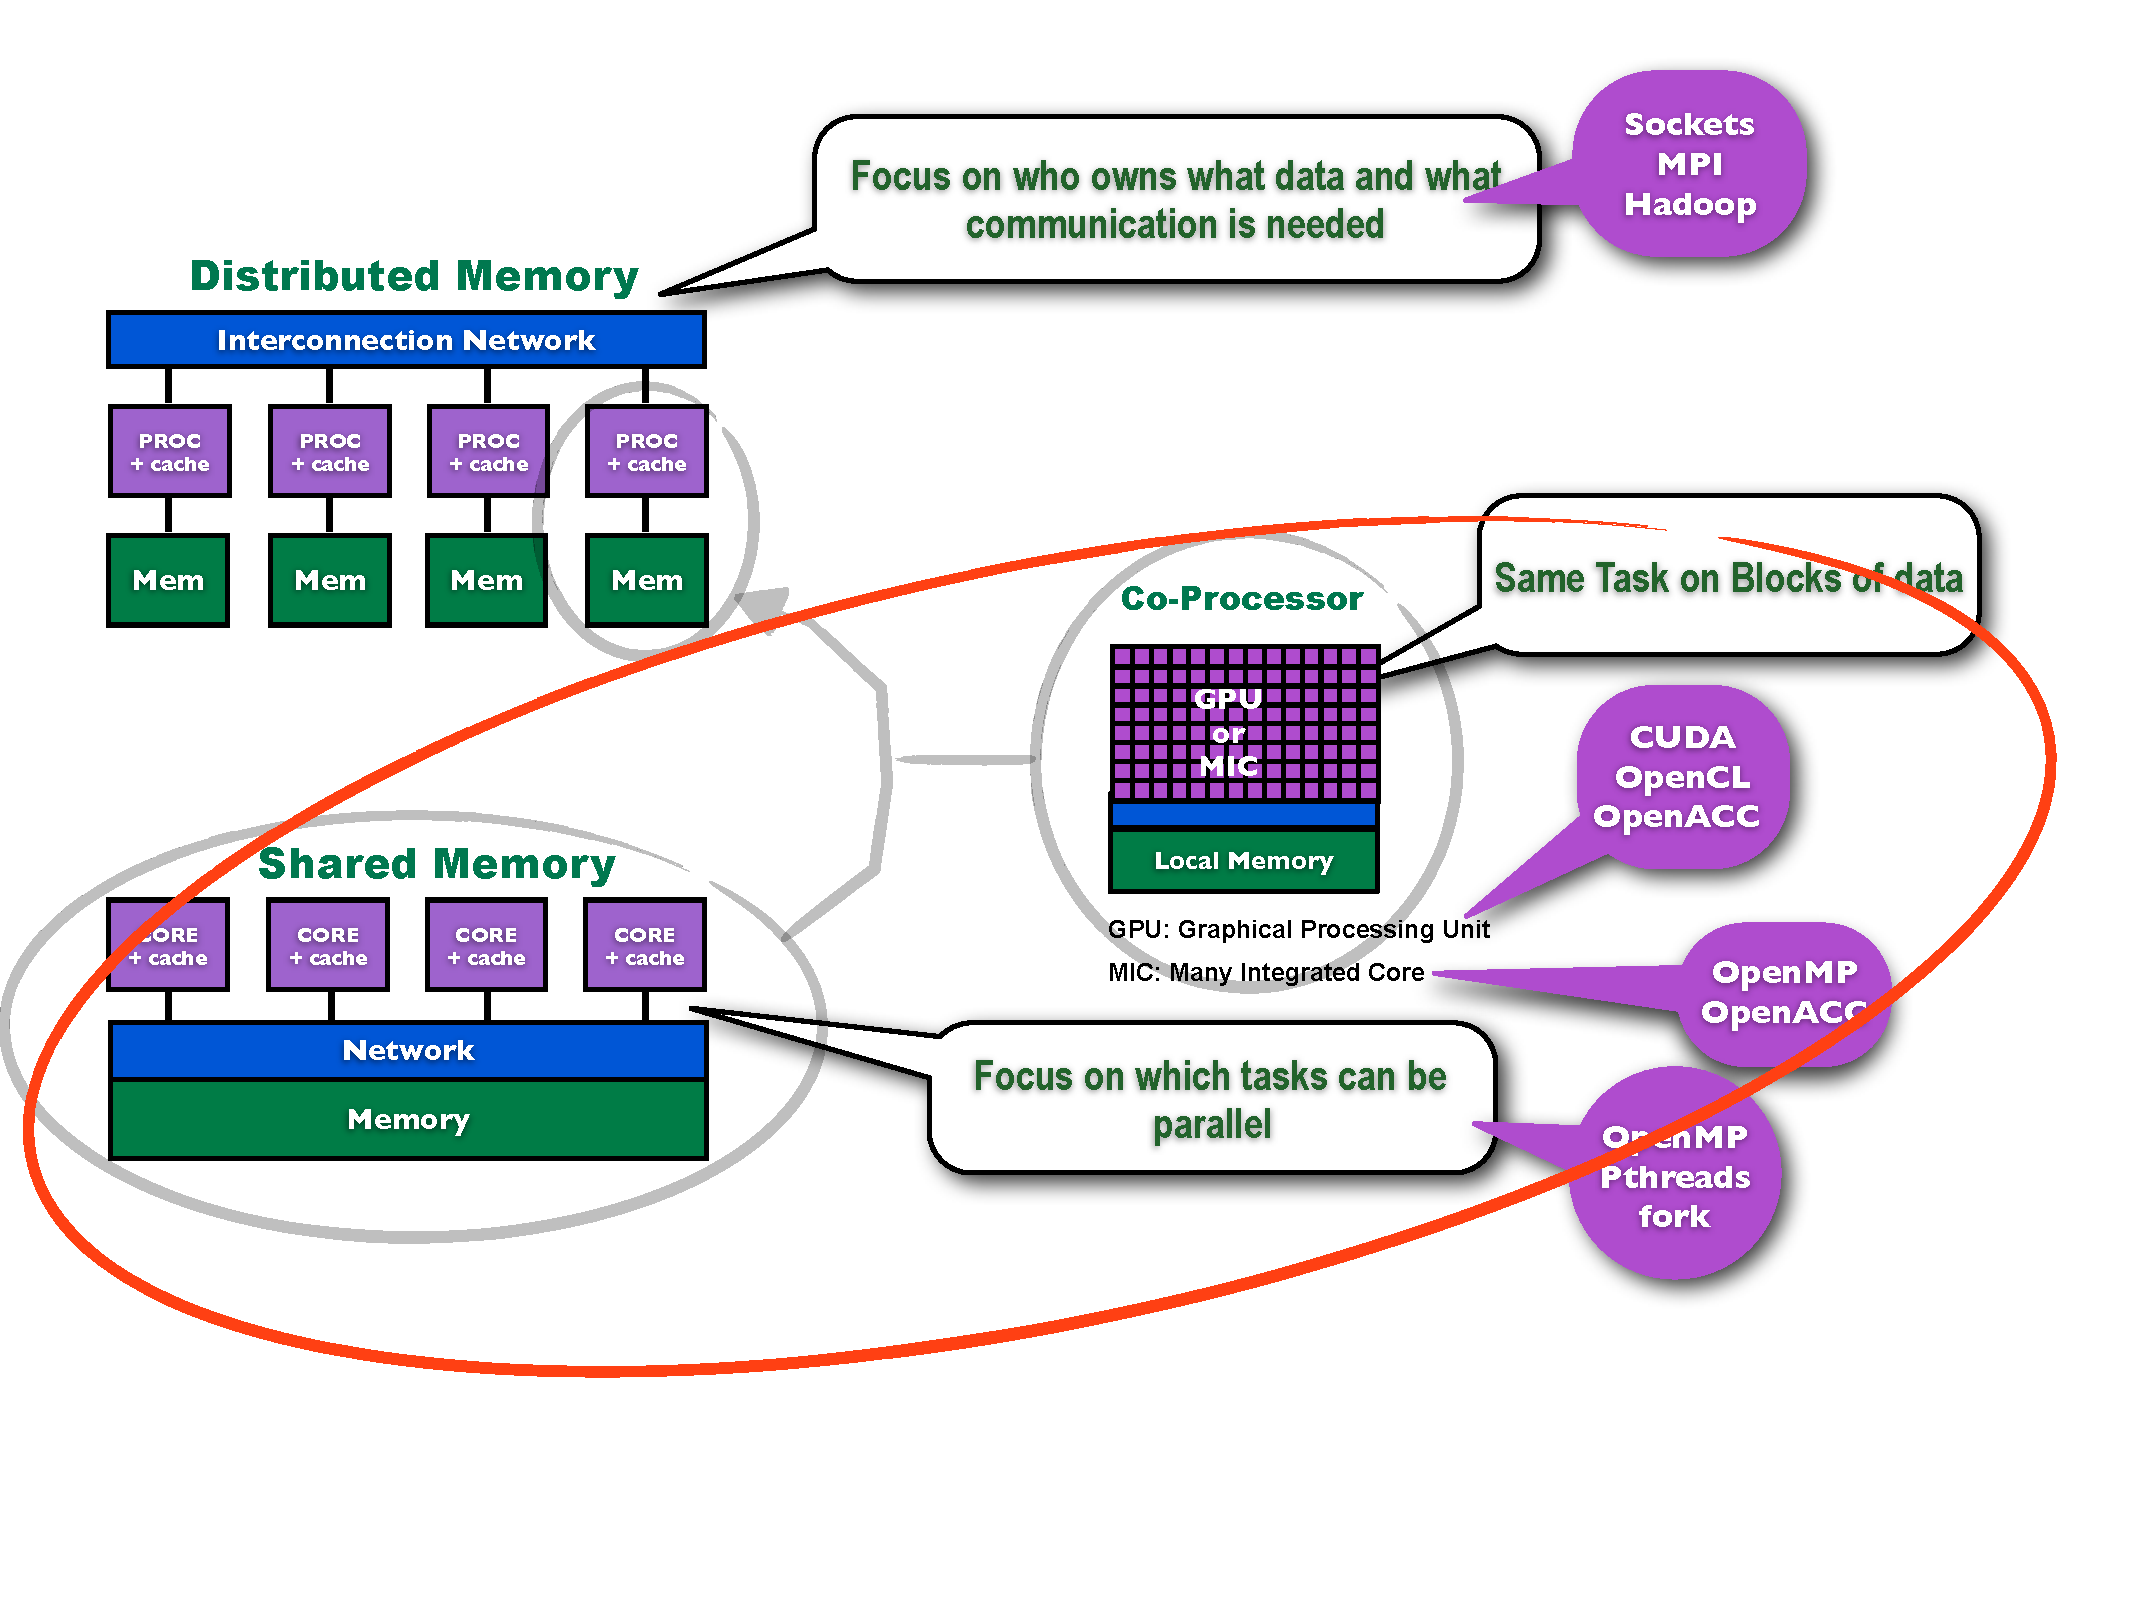
\includegraphics[width=0.95\textwidth]
{../common/pics/hardware/ParallelHardware8.pdf}
\end{block}
\end{frame}

\begin{frame}
\begin{block}{Last 10 years of Advances}
    
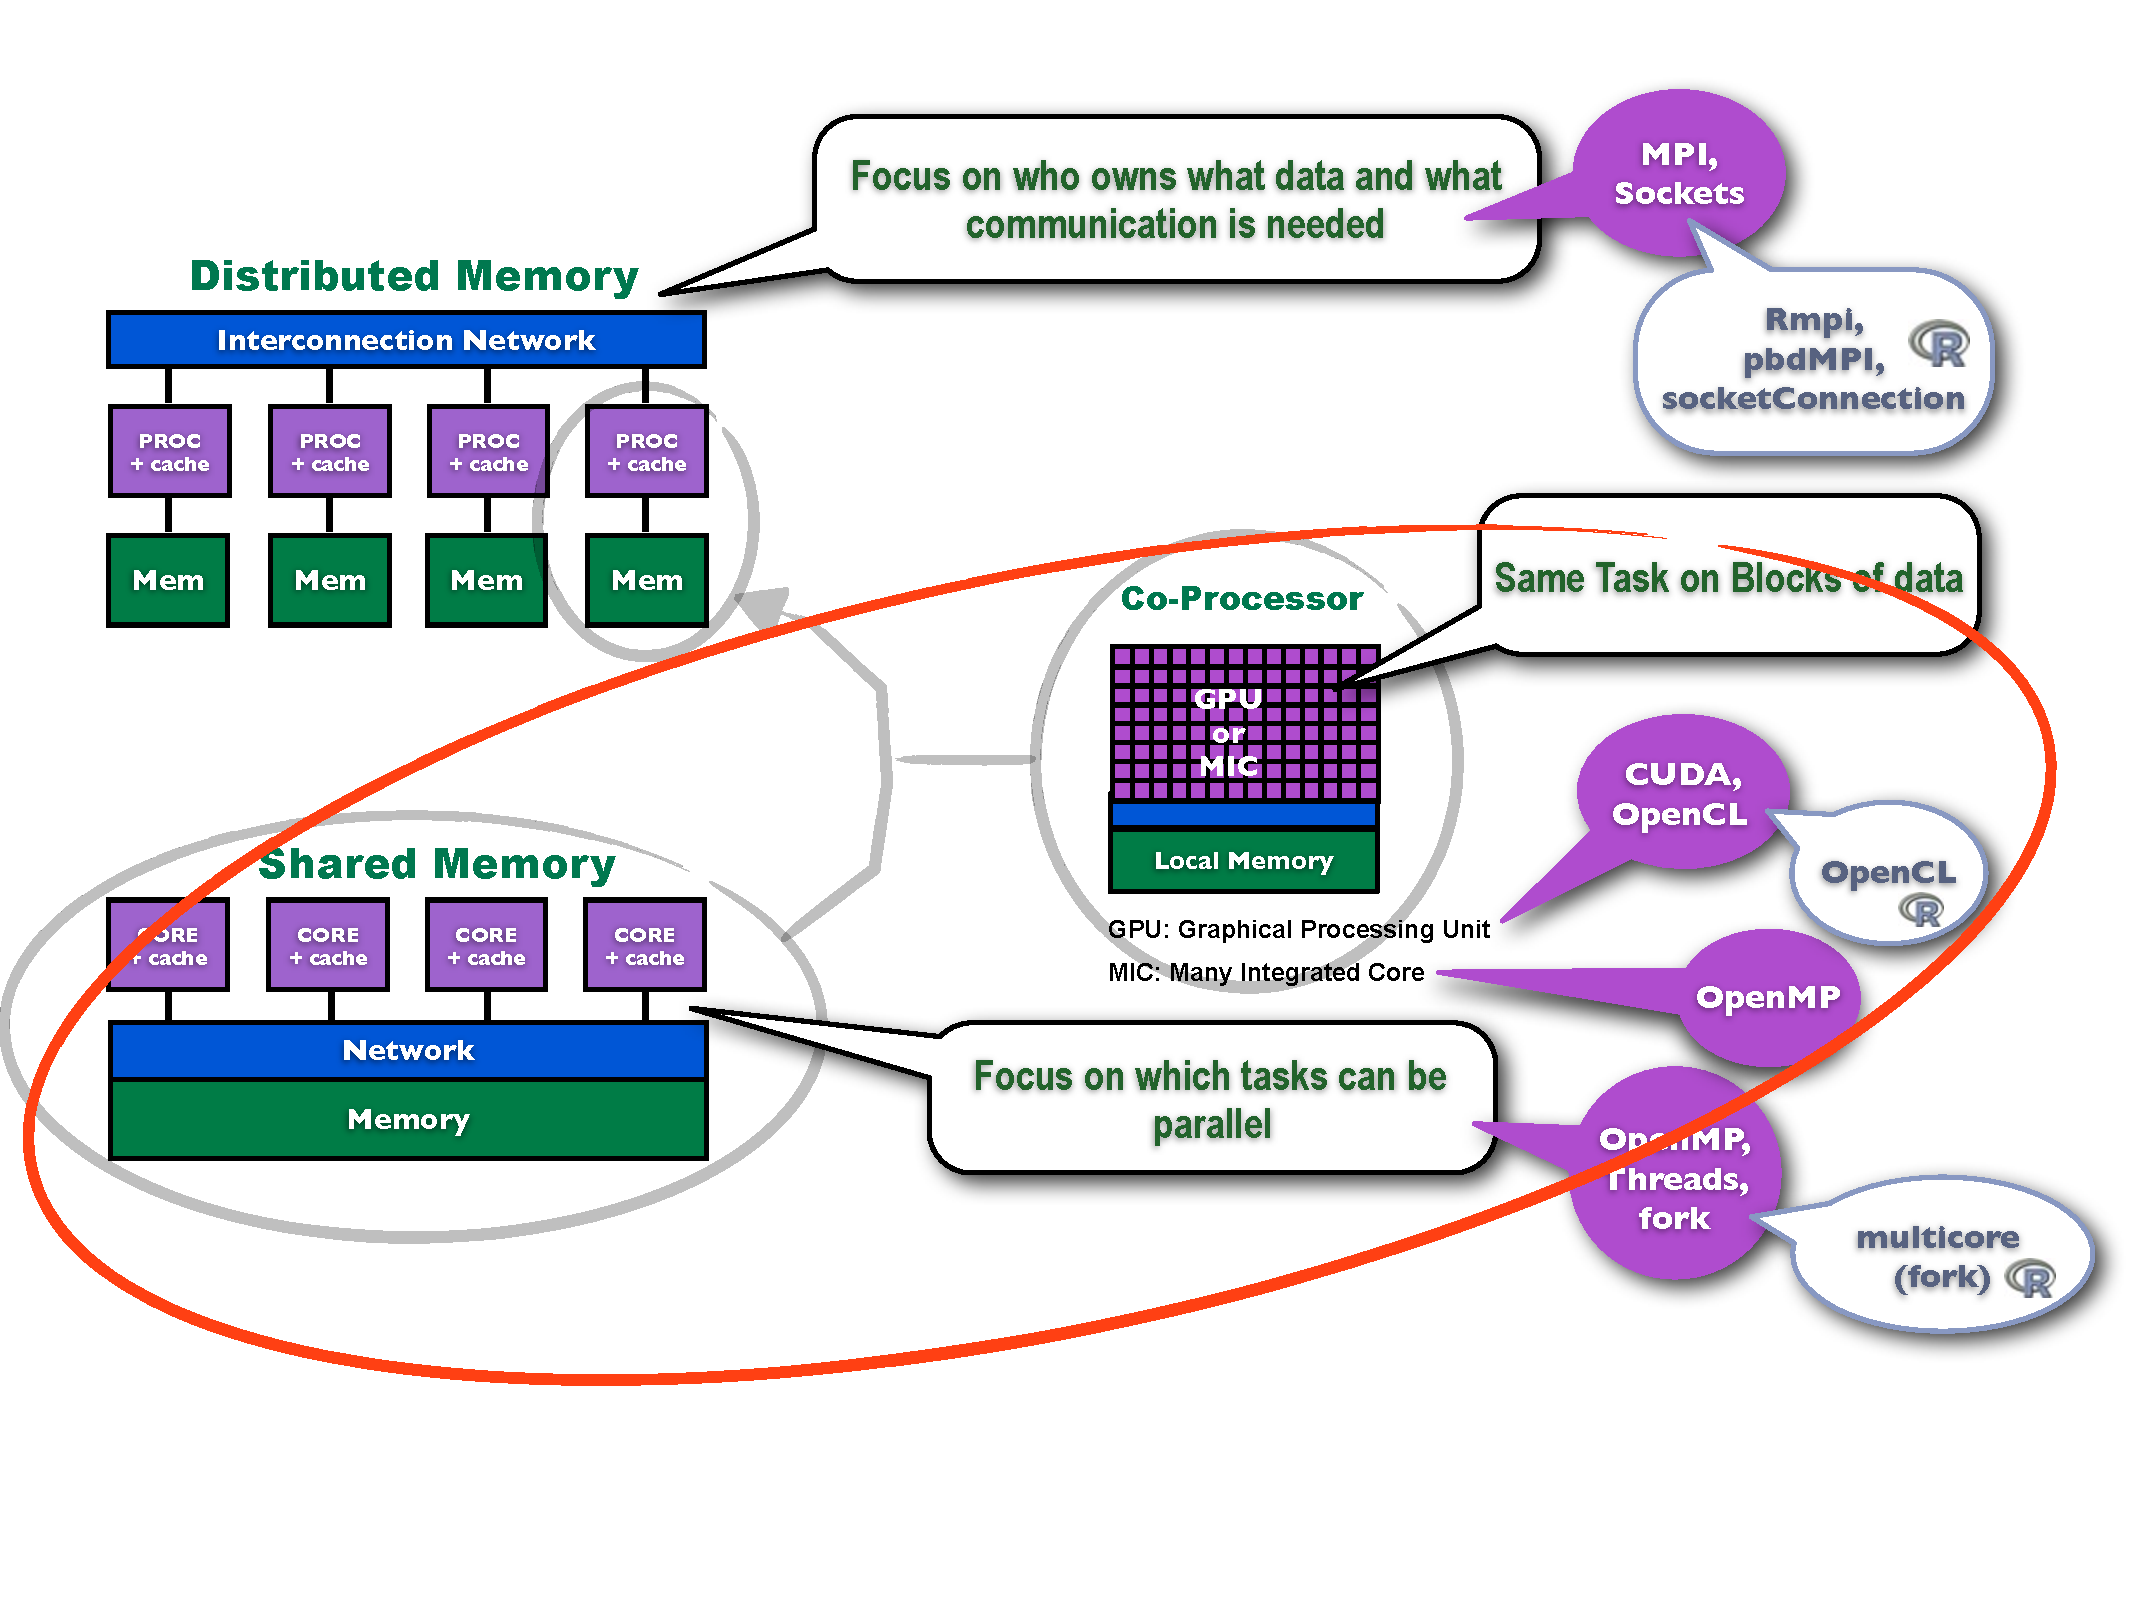
\includegraphics[width=0.95\textwidth]
{../common/pics/hardware/ParallelHardware9.pdf}
\end{block}
\end{frame}

\begin{frame}
\begin{block}{Putting It All Together Challenge}
    
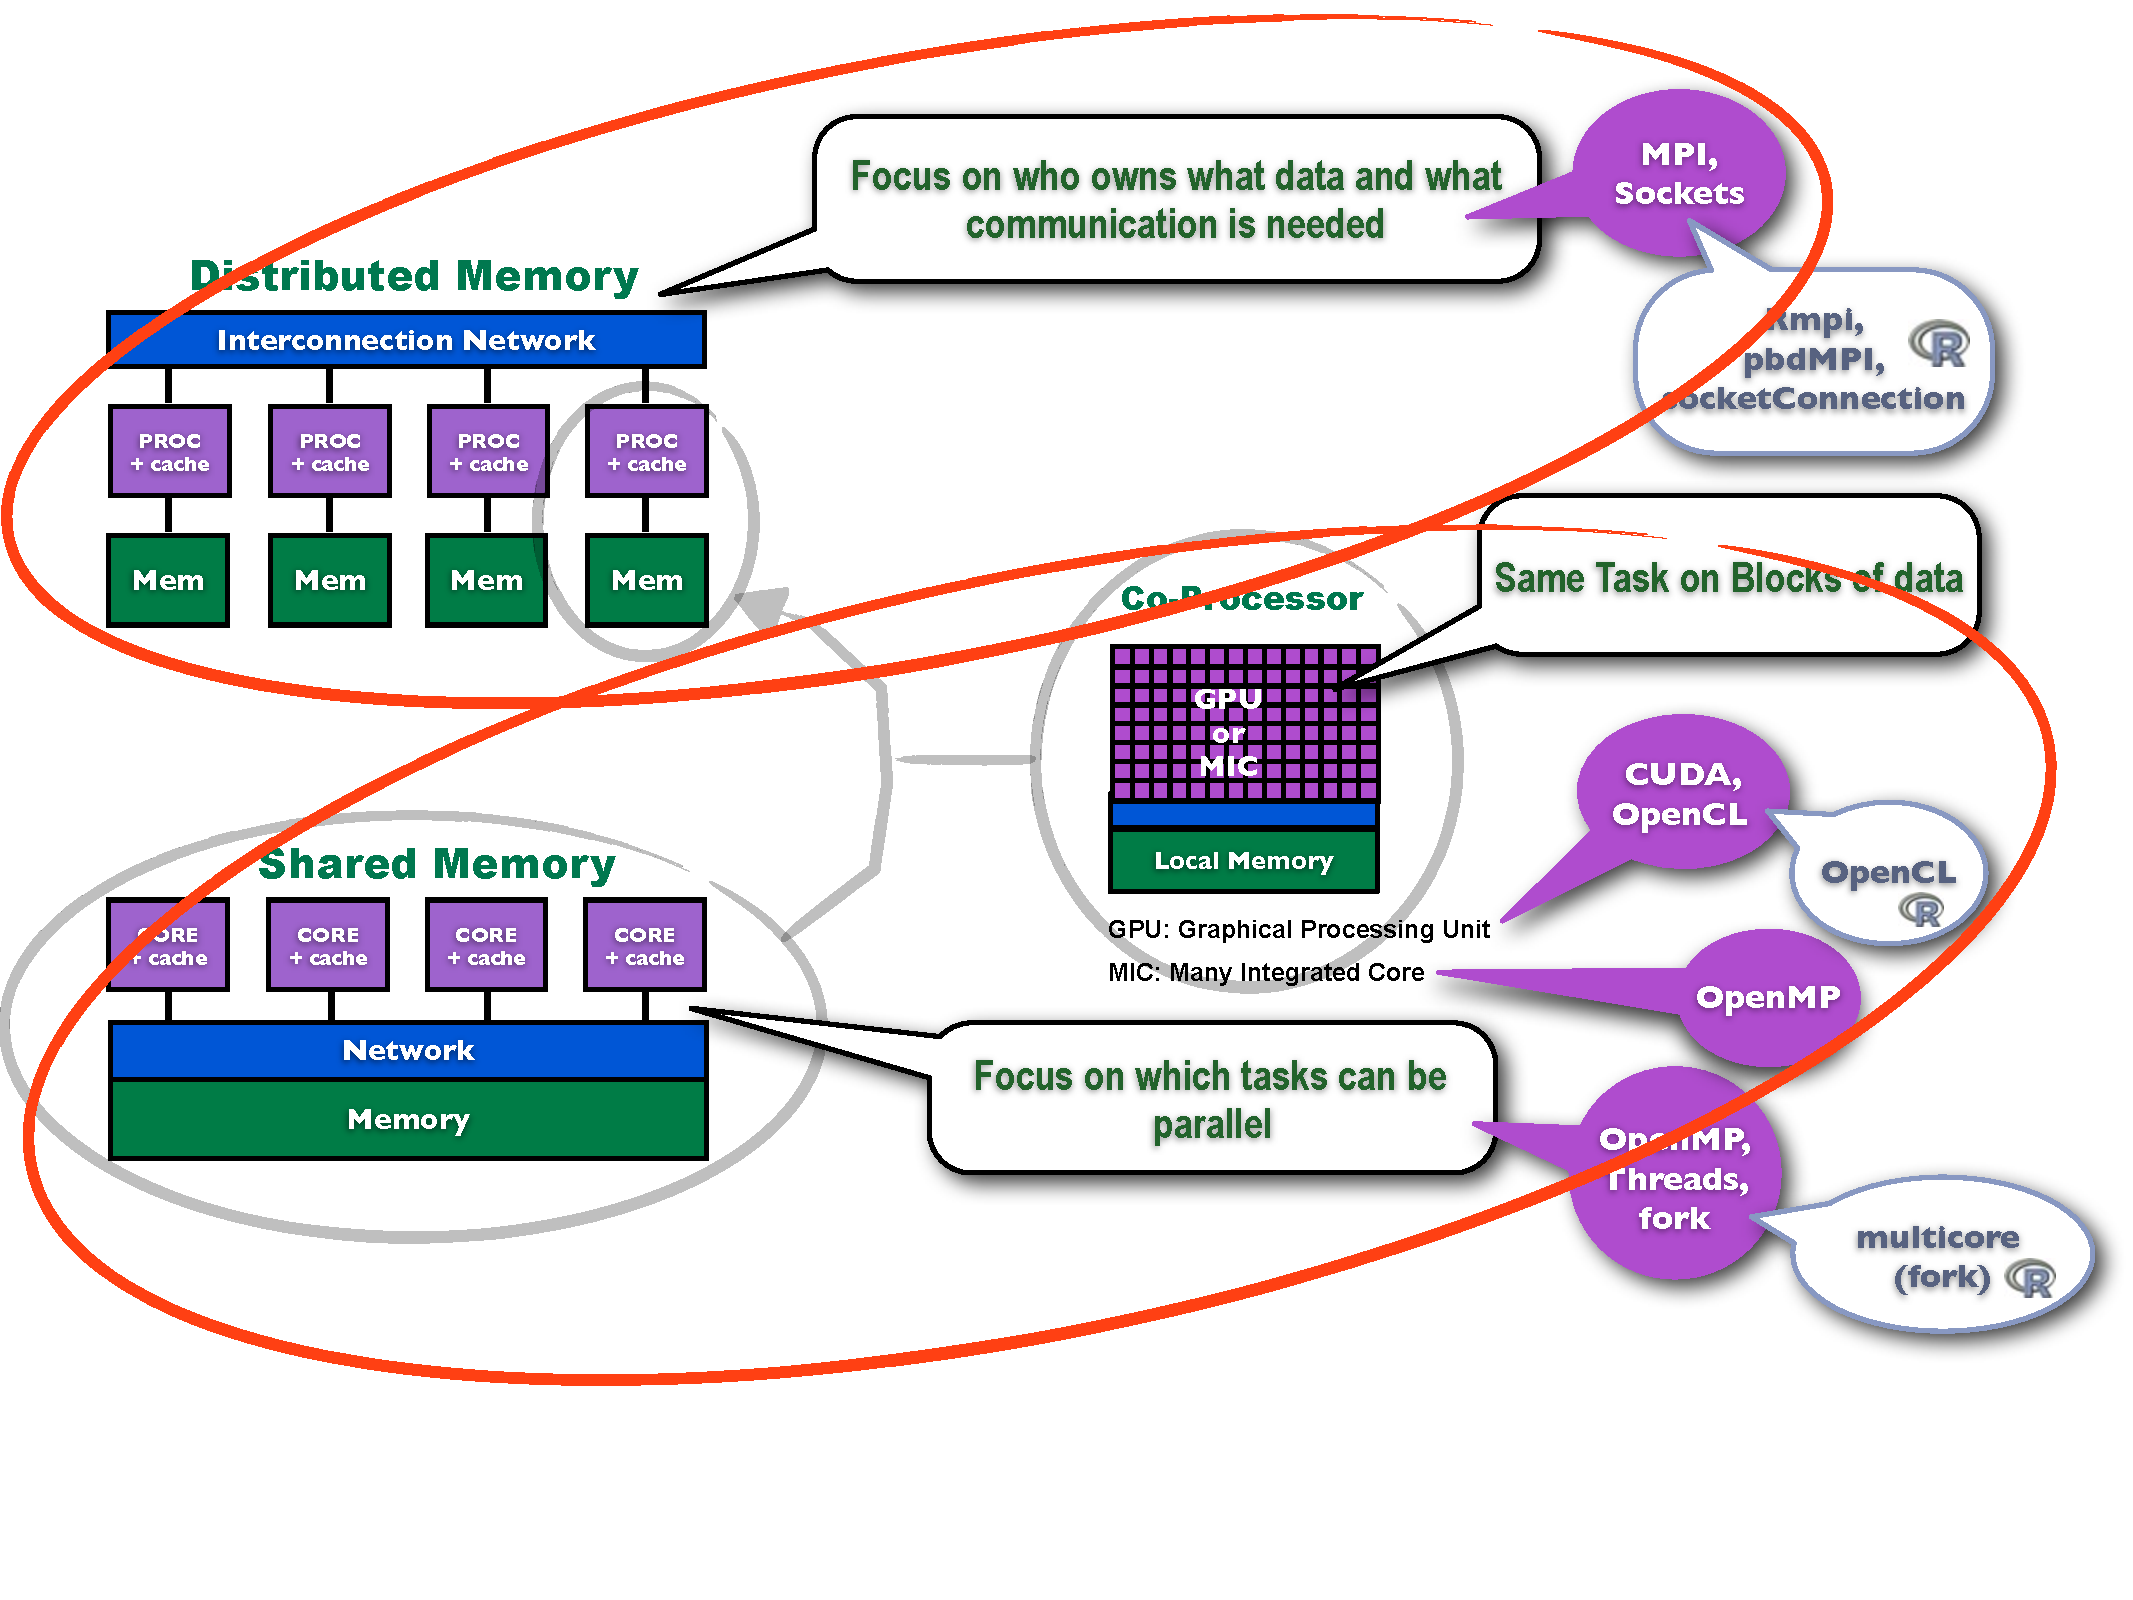
\includegraphics[width=0.95\textwidth]
{../common/pics/hardware/ParallelHardware10.pdf}
\end{block}
\end{frame}

\begin{frame}
\begin{block}{pbdR Focus on Data Parallelism}
    
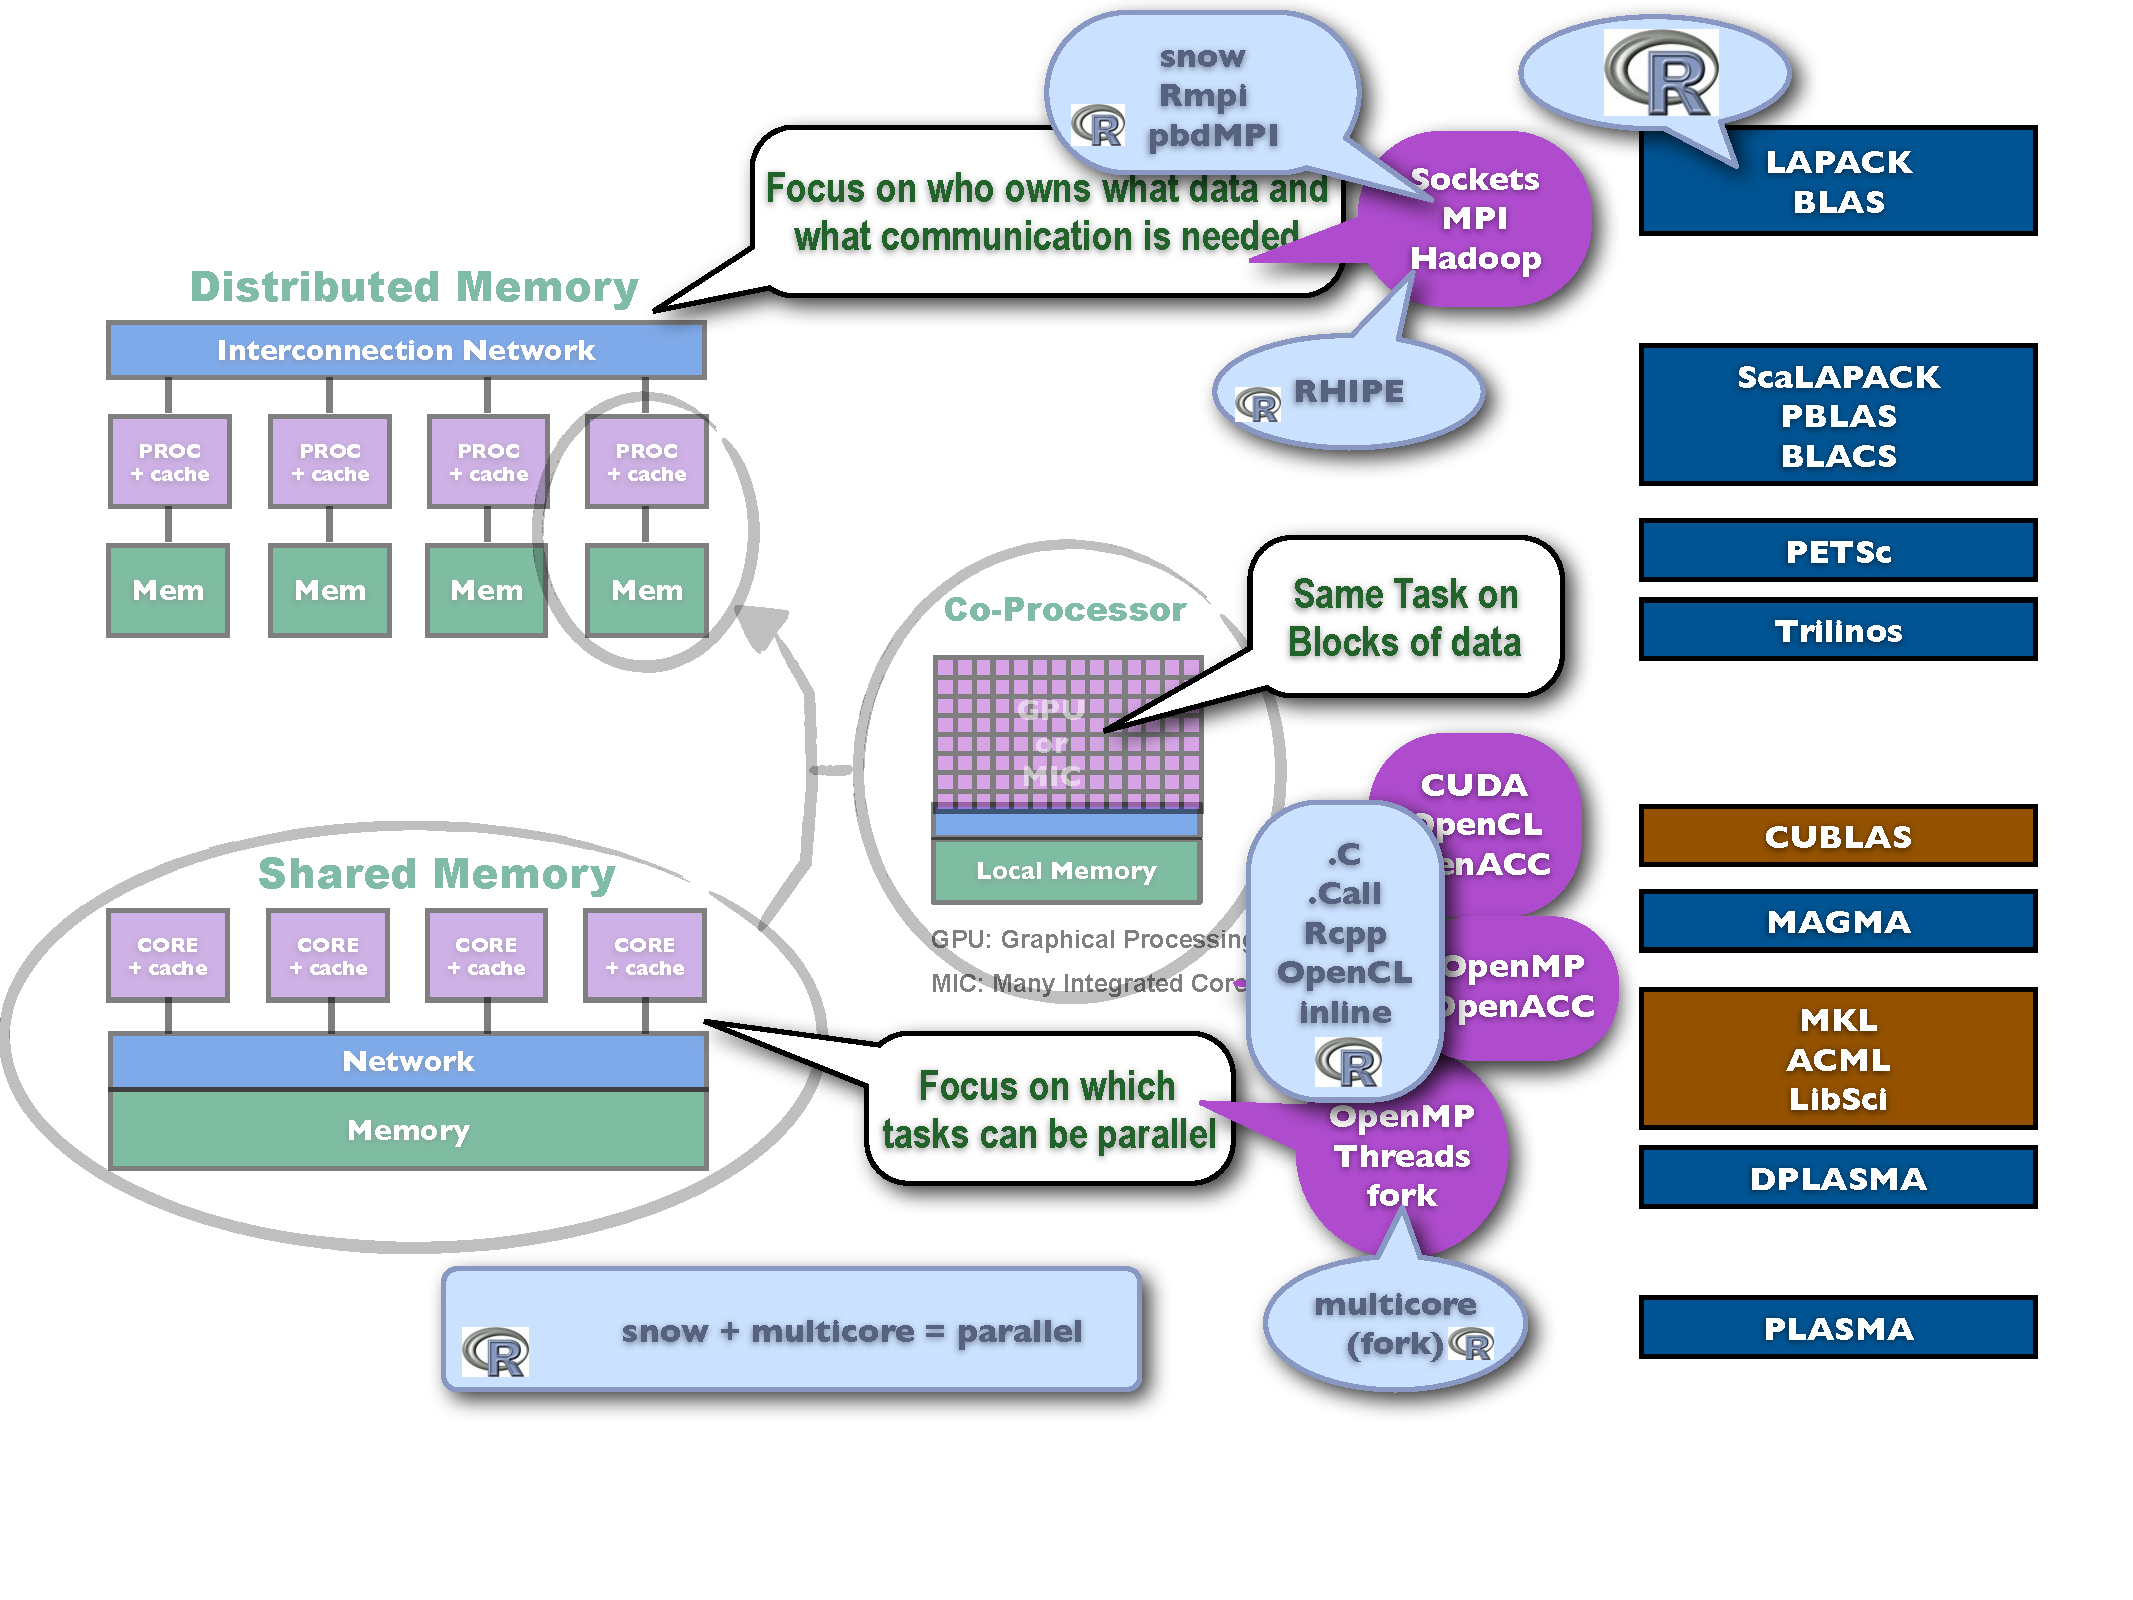
\includegraphics[width=0.95\textwidth]
{../common/pics/hardware/ParallelHardware11.pdf}
\end{block}
\end{frame}